\section{Experimental Details \label{sec:app_exp_details}}

\subsection{Synthetics}
Our synthetic tasks, inspired by~\citep{olsson2022context}, are designed to mimic the in-context learning capability of large language models---the ability to learn from examples in the input sequence, and use information from the input to generate the right answer for the output.
For example, the induction head task requires memorizing the token that appears after the special $\vdash$ token in the input sequence, and the associative recall task requires learning the mapping from keys to tokens from the input sequence.

We evaluate synthetics by training two-layer versions of our GPT models, with different modules replacing attention.
We train models with inner dimension 32, and MLP dimension 128.
For all the synthetics, we use a learning rate of 5e-4 and a weight decay of 0.1.
We sample 5000 training examples and 500 test examples from the same distribution, and we train for 200 epochs.
Again, we use embedding dropout of 0.1 and residual dropout of 0.0.

\subsection{Model Architecture}
For our 125M models, we use 12 layers, with hidden dimension 1024, and MLP dimension 4096.
For our 355M models, we use 24 layers, with the same hidden dimension and MLP dimension.
The 1.3B models have 24 layers, with hidden dimension 2048, and MLP dimension 8192.
The 2.7B models have 32 layers, hidden dimension 2560, and MLP dimension 10240.
The hybrid models have 12, 16, 16, and 20 heads for the 125M, 355M, 1.3B, and 2.7B models, respectively.
The 125M hybrid model has an attention layers at layers 1 and 7, the 355M and 1.3B hybrid models have attention layers at layers 1 and 13, and the 2.7B hybrid model has attention layers at layers 10 and 21.
For both our hybrid models and our \hthree models, we use SSM state size 64.
Our hybrid model uses head dimension 1 for \hthree, while our pure \hthree model uses head dimension 8.
We run models with mixed-precision training, with bf16 for the MLP's and attention.
When training language models, we use fp32 for the FFTConv.

\subsection{OpenWebText Training}
For the 125M models trained on OpenWebText, we follow the training recipe of the Megatron-LM repo.

We use an effective batch size of 512, and use gradient accumulation to fit into
available GPU memory.
We use the AdamW optimizer, with learning rate 6e-4 for GPT-2 small and 1.5e-4
for GPT-2 medium, and weight decay of 0.1.
All models are trained with the same hyperparameters for 100K steps.
We run all implementations with mixed-precision training (PyTorch AMP).
We train models with sequence length 1024.

We use the Openwebtext dataset, with the GPT-2 BPE tokenizer. We randomly select
0.5\% of the dataset as the validation set, with the rest being used as training
set.
This random selection of validation set is done once, and all models are evaluated
on the same validation set.

\subsection{The Pile Training}
For the 125M and 355M models trained on the Pile, we follow the training recipe of GPT-3.
We use batch size 256, with sequence length 2048.
We train our models for 800K steps.
We use residual dropout 0.0 and embedding dropout 0.1.
We use the AdamW optimizer, with learning rate 6e-4 for the 125M model and 3e-4 for the 355M model, and a weight decay of 0.1.
We use a cosine schedule with 8000 steps for linear warmup, and decay the
learning rate to 10\% by 300B tokens, then continue training at 10\% learning
rate for another 100B tokens.
We suspect that there exist better hyperparameters for \hthree language models, but we did not have the resources to tune them.

For the 1.3B models, we double the batch size to 512 (with sequence length
2048), again following the training recipe of GPT-3. The number of training
steps are halved so that we train on the same number of tokens.

For the Pile dataset, we again use the GPT-2 BPE tokenizer, similar to GPT-3 and GPT-Neo.

\subsection{SuperGLUE}
We follow the prompts used in the GPT-3 paper~\citep{brown2020language}.
For rank classification on the binary classification tasks, we use yes/no for WSC, WIC, MultiRC, and BoolQ, and we use true/false for RTE.
For CB, we use true/false/neither as the three choices.
For COPA and ReCoRD, we use the continuations provided by the task.

\subsection{Hardware}
All models were trained on either a single 16xA100-40GB node or a cluster of 8xA100-80GB nodes.

\section{Additional Experiments}
\label{sec:app_additional_experiments}

\subsection{LRA Accuracy}
We evaluate the accuracy of \hthree on LRA.
We compare accuracy to S4D~\citep{gu2022parameterization}, since \hthree uses an S4D kernel as a component in its layer.
We use the same hyperparameters as S4D, and make the layer bidirectional by making two copies and running them in opposite directions.

\begin{table}[ht]
    % \captionsetup{font=small}
    \small
    \centering
    % \vspace{-1em}
    \caption{\label{table:lra_acc} LRA performance of \hthree compared to S4D. }
    %   \vspace{1em}
    {
        \begin{tabular}{@{}|c|cccccc|c|@{}}
            \hline
        %   \specialrule{.15em}{.05em}{.05em}
        Model & ListOps & Text & Retrieval & Image & Pathfinder & Path-X & Avg  \\ % & Training time \\
        %   \specialrule{.15em}{.05em}{.05em}
        \hline
        % GPT-2 small (125M) & -- & -- & -- & -- & -- & -- & -- & -- & -- \\ % & 4.7 days \\
        % H3 (126M) & 18.7 & 4.5 days \\ \hline
        S4D~\citep{gu2022parameterization} & \textbf{58.3} & 87.3 & 90.7 & \textbf{87.5} & \textbf{93.6} & \textbf{92.3} & \textbf{85.0} \\
        \hthree & 57.5 & \textbf{88.2} & \textbf{91.0} & 87.3 & 93.0 & 91.8 & 84.8  \\ \hline
        \end{tabular}
    }
    % \vspace{-1.5em}
\end{table}

Table~\ref{table:lra_acc} shows that \hthree performs well on the LRA benchmark, even thought it was designed for autoregressive language modeling.
\hthree outperforms S4D on two of the LRA tasks, and comes within 1 point on the others.

\subsection{WikiText103}
We train 125M-sized models on WikiText103~\citep{merity2016pointer} and compare their test PPL to transformers, as well as other variants of efficient or long-range attention.
We use the same hyperparameters and setup as training on OpenWebText.
We also provide results from Transformer-XL and Perceiver AR for context, though the results may not be directly comparable due to differences in model size and tokenizer.

\begin{table}[h]
%   \vspace{-1em}
\caption{\label{table:wikitext103} Test PPL on WikiText103.}
\centering
\small
\begin{tabular}{|c|c|}
\hline
Models &  PPL \\
\hline
Transformer (125M) & 18.6  \\
Hybrid \hthree (125M) & 18.5 \\
Performer (125M)~\citep{choromanski2020rethinking} & 26.8 \\
Reformer (125M)~\citep{kitaev2020reformer} & 26.0 \\
Linear Attention (125M)~\citep{katharopoulos2020transformers} & 25.6 \\ \hline
Perceiver AR (358M)~\citep{hawthorne2022general} & 18.4 \\
Transformer-XL (285M)~\citep{dai2019transformer} & 18.4 \\ \hline
% \specialrule{.15em}{.05em}{.05em}
\end{tabular}
%   }
% \vspace{-1em}
\end{table}

Table~\ref{table:wikitext103} shows that the Hybrid \hthree model is competitive with Transformers of the same size, as well as larger models such as the 358M Perceiver AR and 285M Transformer-XL.
The hybrid \hthree model also significantly outperforms transformers with performer, reformer, and linear attention.

We note that the Transformer-XL and Perceiver AR PPl numbers are from the original papers, and may not be directly comparable to our results.
In particular, they use a tokenizer with a different vocab size, which means that the PPLs are not directly comparable.
In addition, the larger vocab size necessitates a change in the model (adaptive softmax) that may affect performance.
The top five numbers in Table~\ref{table:wikitext103} are trained with the same setup and are directly comparable to each other.

\subsection{PG-19}
We evaluate models trained on the PG-19 dataset~\citep{rae2019compressive}, a natural language dataset comprised of texts from books.
We compare the performance of Hybrid \hthree compared against Transformers and linear attention.
We use the same setup as evaluating on OpenWebText.

\begin{table}[h]
%   \vspace{-1em}
\caption{\label{table:pg19} Test PPL on PG-19.}
\centering
\small
\begin{tabular}{|c|c|}
\hline
Models &  PPL \\
\hline
Transformer (125M) & 17.0  \\
Hybrid \hthree (125M) & 16.2 \\
Linear Attention (125M)~\citep{katharopoulos2020transformers} & 19.1 \\ \hline
\end{tabular}
%   }
% \vspace{-1em}
\end{table}

Table~\ref{table:pg19} shows that Hybrid \hthree outperforms transformers and linear attention.

\subsection{Length Extrapolation}
One property of SSMs is that they can naturally extrapolate to sequence lengths longer than those seen during training.
We use the synthetic associative recall task to demonstrate that \hthree maintains this capability.
To do so, we train a two-layer \hthree model on sequences of length 20 drawn from the associative recall synthetic language.
Then, we evaluate accuracy of the last token prediction on sequences of length 20 and 40.

\begin{table}[h]
%   \vspace{-1em}
\caption{\label{table:length_extrapolation} Accuracy of an \hthree model trained for associative recall on sequences of length 20, evaluated on sequences of length 20 and 40.}
\centering
\small
\begin{tabular}{|c|cc|}
\hline
Models & Acc, seqlen 20 & Acc, seqlen 40 \\
\hline
\hthree & 99.8 & 98.4 \\ \hline
\end{tabular}
%   }
% \vspace{-1em}
\end{table}

Table~\ref{table:length_extrapolation} shows that \hthree maintains accuracy on sequences of length 40, which is twice the length of the training sequences.

\subsection{Scaling in Number of Tokens}
We evaluate how well a Hybrid \hthree model scales with the number of tokens seen during training, compared to a Transformer.
For these experiments, we train a 125M Hybrid \hthree model and a 125M Transformer on the Pile for 5B, 10B, and 15B tokens.
We use a learning rate of 6e-4, adjusting the warmup to be 1\% of the total training time, and adjusting the decay rate to decay the learning rate to 6e-5 by the end of training.

\begin{table}[h]
%   \vspace{-1em}
\caption{\label{table:scaling_tokens} Test PPL on the Pile for models trained with fewer tokens.}
\centering
\small
\begin{tabular}{|c|cc|}
\hline
Train Tokens & Hybrid \hthree (125M) & Transformer (125M) \\
\hline
5B & 11.8 & 12.7 \\
10B & 10.7 & 11.3 \\
15B & 10.2 & 10.7 \\
\hline
\end{tabular}
%   }
% \vspace{-1em}
\end{table}

Table~\ref{table:scaling_tokens} shows the results.
Both the Hybrid \hthree model and Transformer model improve as the number of training tokens increases.

\subsection{\hthree Language Model}
\begin{table}[ht]
    % \captionsetup{font=small}
    \small
    \centering
    % \vspace{-1em}
    \caption{\label{table:superglue_zeroshot_all} Zero-shot performance on SuperGLUE with rank classification. Best results for each model size in bold. }
    %   \vspace{1em}
    {
        \begin{tabular}{@{}|c|cccccccc|c|@{}}
            \hline
        %   \specialrule{.15em}{.05em}{.05em}
        Model & WSC & WIC & RTE & CB & MultiRC & ReCoRD & BoolQ & COPA & Average \\ % & Training time \\
        %   \specialrule{.15em}{.05em}{.05em}
        \hline
        % GPT-2 small (125M) & -- & -- & -- & -- & -- & -- & -- & -- & -- \\ % & 4.7 days \\
        % H3 (126M) & 18.7 & 4.5 days \\ \hline
        OPT-125M & \underline{39.4} & \underline{52.0} & 48.7 & 37.4 & \underline{58.9} & \underline{44.9} & \underline{59.6} & \underline{60.0} & 50.1 \\
        GPT-Neo-125M & 36.5 & \textbf{53.6} & \underline{53.1} & \underline{41.1} & \textbf{59.9} & 39.6 & \textbf{62.2} & \underline{60.0} & \underline{50.8} \\
        \textbf{\hthree-125M} & \textbf{61.5} & 50.0 & \underline{53.1} & \underline{41.1} & 4.6 & 15.8 & 46.4 & 51.0 & 40.4 \\%2.7 days
        \textbf{Hybrid \hthree-125M} & \underline{39.4} & 51.4 & \textbf{59.2} & \textbf{48.2} & 51.4 & \textbf{55.0} & \underline{59.6} & \textbf{67.0} & \textbf{53.9} \\ \hline %2.7 days \\ \hline
        \end{tabular}
    }
    % \vspace{-1.5em}
\end{table}
\begin{table}[h]
    % \captionsetup{font=small}
    \small
    \centering
    % \vspace{-1em}
    \caption{\label{table:superglue_fewshot_all} 3-shot performance on SuperGLUE with rank classification. Best results for each size in bold, second best underline. }
    %   \vspace{1em}
    {
        \begin{tabular}{@{}|c|cccccccc|c|@{}}
            \hline
        %   \specialrule{.15em}{.05em}{.05em}
        Model & WSC & WIC & RTE & CB & MultiRC & ReCoRD & BoolQ & COPA & Average \\ % & Training time \\
        %   \specialrule{.15em}{.05em}{.05em}
        \hline
        % GPT-2 small (125M) & -- & -- & -- & -- & -- & -- & -- & -- & -- \\ % & 4.7 days \\
        % H3 (126M) & 18.7 & 4.5 days \\ \hline
        OPT-125M & 36.5 & \textbf{50.2} & 47.3 & 44.6 & \textbf{57.9} & \underline{44.9} & 41.9 & \underline{60.0} & \underline{47.9} \\
        GPT-Neo-125M & 38.5 & \underline{50.0} & \underline{53.1} & 17.9 & \underline{56.3} & 39.6 & \textbf{62.1} & \underline{60.0} & 47.2 \\
        \textbf{\hthree-125M} & \textbf{63.5} & \underline{50.0} & 52.3 & \underline{48.2} & 32.6 & 15.8 & 37.8 & 51.0 & 43.9 \\ %2.7 days \\ \hline
        \textbf{Hybrid \hthree-125M} & \underline{43.3} & 49.1 & \textbf{58.1} & \textbf{51.8} & 48.9 & \textbf{55.0} & \underline{56.1} & \textbf{67.0} & \textbf{53.7} \\ \hline %2.7 days \\ \hline
        \end{tabular}
    }
    % \vspace{-1.5em}
\end{table}

We report the results of a pure \hthree language model on NLP evaluations.
We train a 125M model on the Pile for 400B tokens.
Tables~\ref{table:superglue_zeroshot_all} and~\ref{table:superglue_fewshot_all} show zero-shot and few-shot performance on SuperGLUE, respectively.

\subsection{Generation Performance\label{sec:app_generation}}
\begin{table}[h]
    % \captionsetup{font=small}
    \scriptsize
    \centering
    % \vspace{-1em}
    \caption{\label{table:superglue_zeroshot} Zero-shot performance on SuperGLUE. Best results for each size in bold, second best underline. }
    %   \vspace{1em}
    {
        \begin{tabular}{@{}|c|cccccccc|c|@{}}
            \hline
        %   \specialrule{.15em}{.05em}{.05em}
        Model & WSC & WIC & RTE & CB & MultiRC & ReCoRD & BoolQ & COPA & Average \\ % & Training time \\
        %   \specialrule{.15em}{.05em}{.05em}
        \hline
        % GPT-2 small (125M) & -- & -- & -- & -- & -- & -- & -- & -- & -- \\ % & 4.7 days \\
        % H3 (126M) & 18.7 & 4.5 days \\ \hline
        OPT-125M & \textbf{36.5} & \textbf{48.4} & \textbf{49.8} & \textbf{8.9} & \textbf{39.1} & \underline{44.9} & 45.9 & \underline{60.0} & \textbf{41.7} \\
        GPT-Neo-125M & \underline{27.9} & \underline{11.3} & 45.8 & \textbf{8.9} & \underline{19.1} & 39.6 & \textbf{56.4} & \underline{60.0} & \underline{33.6} \\
        % \textbf{\hthree-125M} & 0.0 & 0.0 & 47.3 & 8.9 & 0.0 & -- & 37.8 & 51.0 & 20.7 \\ %2.7 days \\ \hline
        \textbf{Hybrid \hthree-125M} & 0.0 & 0.0 & \underline{47.3} & \textbf{8.9} & 4.4 & \textbf{55.0} & \underline{47.6} & \textbf{67.0} & 28.8 \\ \hline %2.7 days \\ \hline
        GPT-2 medium (355M) & \textbf{50.0} & \textbf{50.2} & 16.2 & \textbf{21.4} & 10.5 & \underline{53.3} & 38.4 & \underline{65.0} & \underline{38.1} \\
        % H3 (361M) &  &  \\ \hline
        OPT-350M & \underline{41.3} & \underline{34.8} & \textbf{49.5} & \underline{16.1} & \textbf{23.6} & 51.4 & \underline{39.7} & 60.0 & \textbf{39.6} \\
        \textbf{Hybrid \hthree-355M} & 22.1 & 21.5 & \underline{47.3} & 8.9 & \underline{17.1} & \textbf{62.3} & \textbf{44.4} & \textbf{69.0} & 36.6 \\ \hline
        % GPT-2 (1.5B) & 14.4 & \textbf{36.5} & \underline{49.1} & \underline{8.9} & 0.5 & \underline{44.0} & \underline{46.6} & 59.0 & 32.4 \\
        % OPT-1.3B & \underline{36.5} & \underline{32.0} & 46.9 & \underline{8.9} & \textbf{55.8} & \textbf{61.8} & 37.9 & \underline{69.0} & 43.6 \\
        % GPT-Neo-1.3B & \textbf{39.4} & 22.4 & \textbf{54.9} & \textbf{26.8} & 5.6 & -- & 45.4 & 66.0 & -- \\
        % \textbf{Hybrid \hthree-1.3B} & 30.8 & 0.0 & 47.3 & \underline{8.9} & \underline{19.7} & -- & \textbf{52.5} & \textbf{70.0} & -- \\ \hline
        \end{tabular}
    }
    % \vspace{-1.5em}
\end{table}
\begin{table}[h]
    % \captionsetup{font=small}
    \scriptsize
    \centering
    % \vspace{-1em}
    \caption{\label{table:superglue_fewshot} 3-shot performance on SuperGLUE with generation. Best results for each size in bold, second best underline. }
    %   \vspace{1em}
    {
        \begin{tabular}{@{}|c|cccccccc|c|@{}}
            \hline
        %   \specialrule{.15em}{.05em}{.05em}
        Model & WSC & WIC & RTE & CB & MultiRC & ReCoRD & BoolQ & COPA & Average \\ % & Training time \\
        %   \specialrule{.15em}{.05em}{.05em}
        \hline
        % GPT-2 small (125M) & -- & -- & -- & -- & -- & -- & -- & -- & -- \\ % & 4.7 days \\
        % H3 (126M) & 18.7 & 4.5 days \\ \hline
        OPT-125M & 36.5 & \underline{49.1} & 47.3 & 33.9 & \underline{35.5} & \underline{44.8} & 38.5 & 60.0 & 43.2 \\
        GPT-Neo-125M & \underline{38.5} & \textbf{50.0} & \underline{53.1} & \textbf{42.9} & 22.5 & 39.7 & \textbf{61.2} & \textbf{68.0} & \underline{47.0} \\
        \textbf{\hthree-125M} & 0.0 & 0.0 & 47.3 & 8.9 & 0.0 & 15.4 & 37.8 & 53.0 & 20.3 \\ %2.7 days \\ \hline
        \textbf{Hybrid \hthree-125M} & \textbf{43.3} & \underline{49.1} & \textbf{58.1} & \underline{41.1} & \textbf{40.3} & \textbf{55.2} & \underline{49.5} & \underline{67.0} & \textbf{50.5} \\ \hline %2.7 days \\ \hline
        GPT-2 medium (355M) & 36.5 & \textbf{50.5} & 47.3 & 28.6 & 35.3 & \underline{53.1} & \underline{37.8} & \underline{63.0} & 44.0 \\
        % H3 (361M) &  &  \\ \hline
        OPT-350M & \underline{37.5} & \underline{50.0} & \underline{46.2} & \textbf{41.1} & \underline{40.6} & 51.3 & 39.4 & 59.0 & \underline{45.6} \\
        \textbf{Hybrid \hthree-355M} & \textbf{42.3} & 47.5 & \textbf{50.5} & \underline{37.5} & \textbf{57.5} & \textbf{61.4} & \textbf{45.4} & \textbf{73.0} & \textbf{51.9} \\ \hline
        % GPT-2 (1.5B) & \underline{36.5} & 36.5 & \textbf{56.7} & 41.1 & 6.1 & 43.8 & \underline{53.7} & 61.0 & 41.9 \\
        % OPT-1.3B & \textbf{44.2} & 48.9 & \underline{53.1} & \textbf{55.4} & \underline{58.6} & 62.1 & 37.8 & \underline{70.0} & 53.7 \\
        % GPT-Neo-1.3B & 35.6 & \underline{50.6} & 47.3 & \underline{48.2} & 51.5 & -- & 38.0 & 67.0 & -- \\
        % \textbf{Hybrid \hthree-1.3B} & \underline{36.5} & \textbf{51.3} & 40.8 & 44.6 & \textbf{59.9} & -- & \textbf{56.5} & \textbf{72.0} & -- \\ \hline
        \end{tabular}
    }
    % \vspace{-1.5em}
\end{table}
We report results on SuperGLUE for generation.
Instead of taking rank classification, we instead let the model generate a response, and we search for the gold label (i.e., ``yes'' or ``no'' for the yes/no questions) in the output.
Tables~\ref{table:superglue_zeroshot} and~\ref{table:superglue_fewshot} report the results.
The trends for few-shot learning match with the logit results, but the hybrid and \hthree models perform very poorly in zero-shot performance on some tasks.
In these cases, the models tend to generate long text responses that are not relevant to the answer.
The few-shot learning examples help the models generate answers in a parsable format.

\subsection{Non-Text Sequence Modeling}
\label{subsec:non_text_sequence_modeling}

We show that \hthree outperforms Transformers on two non-text sequence modeling tasks: raw speech classification and seizure classification over raw EEG signals.
\hthree sets state-of-the-art performance on seizure classification and matches S4 on speech classification---which suggests that \hthree, or one of its hybrids, may be a strong candidate for a multimodal foundation model.
Appendix~\ref{sec:app_exp_details} gives experimental details, and Appendix~\ref{sec:app_additional_experiments} gives an additional experiment on brain fMRI data.

\paragraph{Seizure Classification from EEG}
Seizures, which are characterized by uncontrolled brain activity, are some of the most common neurological disorders~\citep{fisher2014ilae}. Chronic seizures, or epilepsy, cause a range of psychiatric and psycho-social disorders and impact the lives of roughly one percent of the global population~\citep{kerr2012impact}. The first step to treating epilepsy is manual analysis of scalp EEG by board-certified neurologists. However, the vast amount of EEG data produced by each patient (which can be up to days of data) makes manual EEG analysis a costly and time-consuming process.  

To mitigate the costs associated with EEG monitoring, recent deep learning techniques have began to show promise in flagging abnormal EEG segments for potential seizure events~\citep{siddiqui2020review}. A challenge with classifying EEG data is the trade-off between increasing input sequence length, where more context has been shown to improve seizure classification performance \cite{saab2020weak}, with the increased difficulty of training deep learning models on long sequences (e.g., an EEG signal sampled at $200$Hz produces $12{,}000$ time steps per minute). As a result, many techniques involve domain-specialized models and pre-processing steps, such as FFT transforms and graphical representations \cite{tang2021self}.

We use the largest publicly available EEG corpus, TUSZ v1.5.2~\citep{shah2018temple}, which includes $5{,}612$ EEG signals from 636 patients, with $3{,}050$ annotated seizures.
Signals are segmented into 60-second clips, and split into train/val/test by patient.
The train set contains 39765 clips, the val set contains 4351 clips, and the test set contains 10001 clips.

\begin{table}[h]
    % \captionsetup{font=small}
    \small
    \centering
    % \vspace{-1em}
    \caption{\label{table:eeg} Performance (AUROC) on 60s seizure classification from raw EEG (sequence length 12000).}
    %   \vspace{1em}
    {
        \begin{tabular}{@{}|cccccc|@{}}
        %   \specialrule{.15em}{.05em}{.05em}
        \hline
        H3 & Transformer  & Dense-CNN & CNN-LSTM & LSTM & 1D-CNN  \\ % & Training time \\
        %   \specialrule{.15em}{.05em}{.05em}
        \hline
        \textbf{83.2} & x  & 78.0 & 68.6 & 69.3 & 69.7 \\
        % FFT Preprocessing & -- & -- & 0.804 & 0.796 & 0.766 & 0.779 & 0.814 \\
        \hline
        \end{tabular}
    }
    % \vspace{-1.5em}
\end{table}

We evaluate binary seizure classification of $60$-sec EEG clips, sampled at $200$Hz, with 19 electrodes: $ x \in R^{12{,}000 \times 19}$ and $y \in \{0,1\}$ on the TUSZ v1.5.2~\citep{shah2018temple} corpus.
Transformers cannot process the long sequence length of EEG signals without running out of GPU memory, whereas \hthree can---and sets state-of-the-art performance.

\paragraph{Raw Speech Classification}
The SC10 speech commands task~\citep{warden2018speech} contains raw audio signals one second in length, sampled at 16kHz.
Similarly to EEG signals, Transformers cannot process the long sequence length.
Table~\ref{table:speech} shows that \hthree comes within half a point of S4, the state-of-the-art method.



\subsection{Speech Understanding Results}
\label{section:results_speech}
We evaluate the speech understanding capabilities of our speech interface for Llama 3 on three tasks: \textbf{(1)} automatic speech recognition, \textbf{(2)} speech translation, and \textbf{(3)} spoken question answering.
We compare the performance of our speech interface for Llama 3 with three state-of-the-art models for speech understanding: Whisper \citep{radford23whisper}, SeamlessM4T \citep{barrault2023seamless}, and Gemini.\footnote{
	Due to technical limitations, we compare with the performance of Gemini on MLS reported in the original paper.
}
In all the evaluations, we used greedy search for Llama 3 token prediction.

\textbf{Speech recognition.}
We evaluate the ASR performance on the
English datasets of
Multilingual LibriSpeech (MLS; \citet{pratap2020mls}),
LibriSpeech \citep{panayotov2015librispeech},
VoxPopuli \citep{wang2021voxpopuli},
and a subset of the multilingual FLEURS dataset \citep{conneau2023fleurs}.
In evaluation, the decoding results are post-processed using the Whisper text normalizer to ensure consistency in comparing with the reported results of other models.
On all benchmarks, we measure the word error rate of our speech interface for Llama 3 on the standard test set of those benchmarks, except for Chinese, Japanese, Korean and Thai, where the character error rate is reported.



\providecommand{\bup}{($\boldsymbol\uparrow$)}
\providecommand{\bdown}{($\boldsymbol\downarrow$)}


\begin{table}[t]
	\centering
	 \resizebox{\linewidth}{!}{\begin{NiceTabular}{lcccccc}
	\CodeBefore
	\Body
	\toprule
	& \textbf{Llama 3 8B} & \textbf{Llama 3 70B} & \textbf{Whisper} & \textbf{SeamlessM4T v2} & \textbf{Gemini 1.0 Ultra} & \textbf{Gemini 1.5 Pro}\\
	\midrule
	MLS \scriptsize{(English)} & 4.9 & 4.4 & 6.2 \scriptsize{(v2)} & 6.5 & 4.4 & \textbf{4.2} \\
	LibriSpeech \scriptsize{(test-other)} & 3.4 & \textbf{3.1} & 4.9 \scriptsize{(v2)} & 6.2 & -- &  -- \\
	VoxPopuli \scriptsize{(English)}  & 6.2 & \textbf{5.7} &  7.0  \scriptsize{(v2)} & 7.0 & -- & --  \\
	FLEURS \scriptsize{(34 languages)} & 9.6 & \textbf{8.2} & 14.4 \scriptsize{(v3)}  & 11.7 & -- & -- \\
	\bottomrule
\end{NiceTabular}
}
	\caption{\textbf{Word error rate of our speech interface for Llama 3 on speech recognition tasks.} We report the performance of Whisper, SeamlessM4T, and Gemini for reference.}
	\label{table:speech_asr_results}
\end{table}


Table~\ref{table:speech_asr_results} shows the results of ASR evaluations.
It demonstrates the strong performance of Llama 3 (and multi-modal foundation models more generally) on speech recognition tasks: our model outperforms models that are tailored to speech like Whisper\footnote{On FLEURS ASR, Malayalam is not officially reported for Whisper v3, so we use the average of 33 languages.} and SeamlessM4T on all benchmarks.
On MLS English, Llama 3 performs similarly to Gemini.


\begin{table}[t]
	\centering
	\begin{NiceTabular}{lcccc}
	\CodeBefore
	\Body
	\toprule
	& \textbf{Llama 3 8B} & \textbf{Llama 3 70B} & \textbf{Whisper v2} & \textbf{SeamlessM4T v2}\\
	\midrule
	FLEURS \scriptsize{(33 lang. $\rightarrow$ English)} & 29.5 & \textbf{33.7}  & 21.9  & 28.6  \\
	Covost 2 \scriptsize{(15 lang. $\rightarrow$ English)} & 34.4 & \textbf{38.8} & 33.8  & 37.9 \\
	\bottomrule
\end{NiceTabular}

	\caption{\textbf{BLEU score of our speech interface for Llama 3 on speech translation tasks.} We report the performance of Whisper and SeamlessM4T for reference.}
	\label{table:speech_ast_results}
\end{table}


\textbf{Speech translation.}
We also evaluate our models on speech translation tasks in which the model is asked to translate non-English speech into English text.
We use the FLEURS and Covost 2 \citep{wang2021covost} datasets in these evaluations, measuring BLEU scores of the translated English.
Table~\ref{table:speech_ast_results} presents the results of these experiments.\footnote{On Covost 2, we evaluate only on 15 (out of 21) languages.} 
The performance of our models in speech translation highlights the advantages of multimodal foundation models for tasks such as speech translation. 

\begin{figure}[]
    \centering
    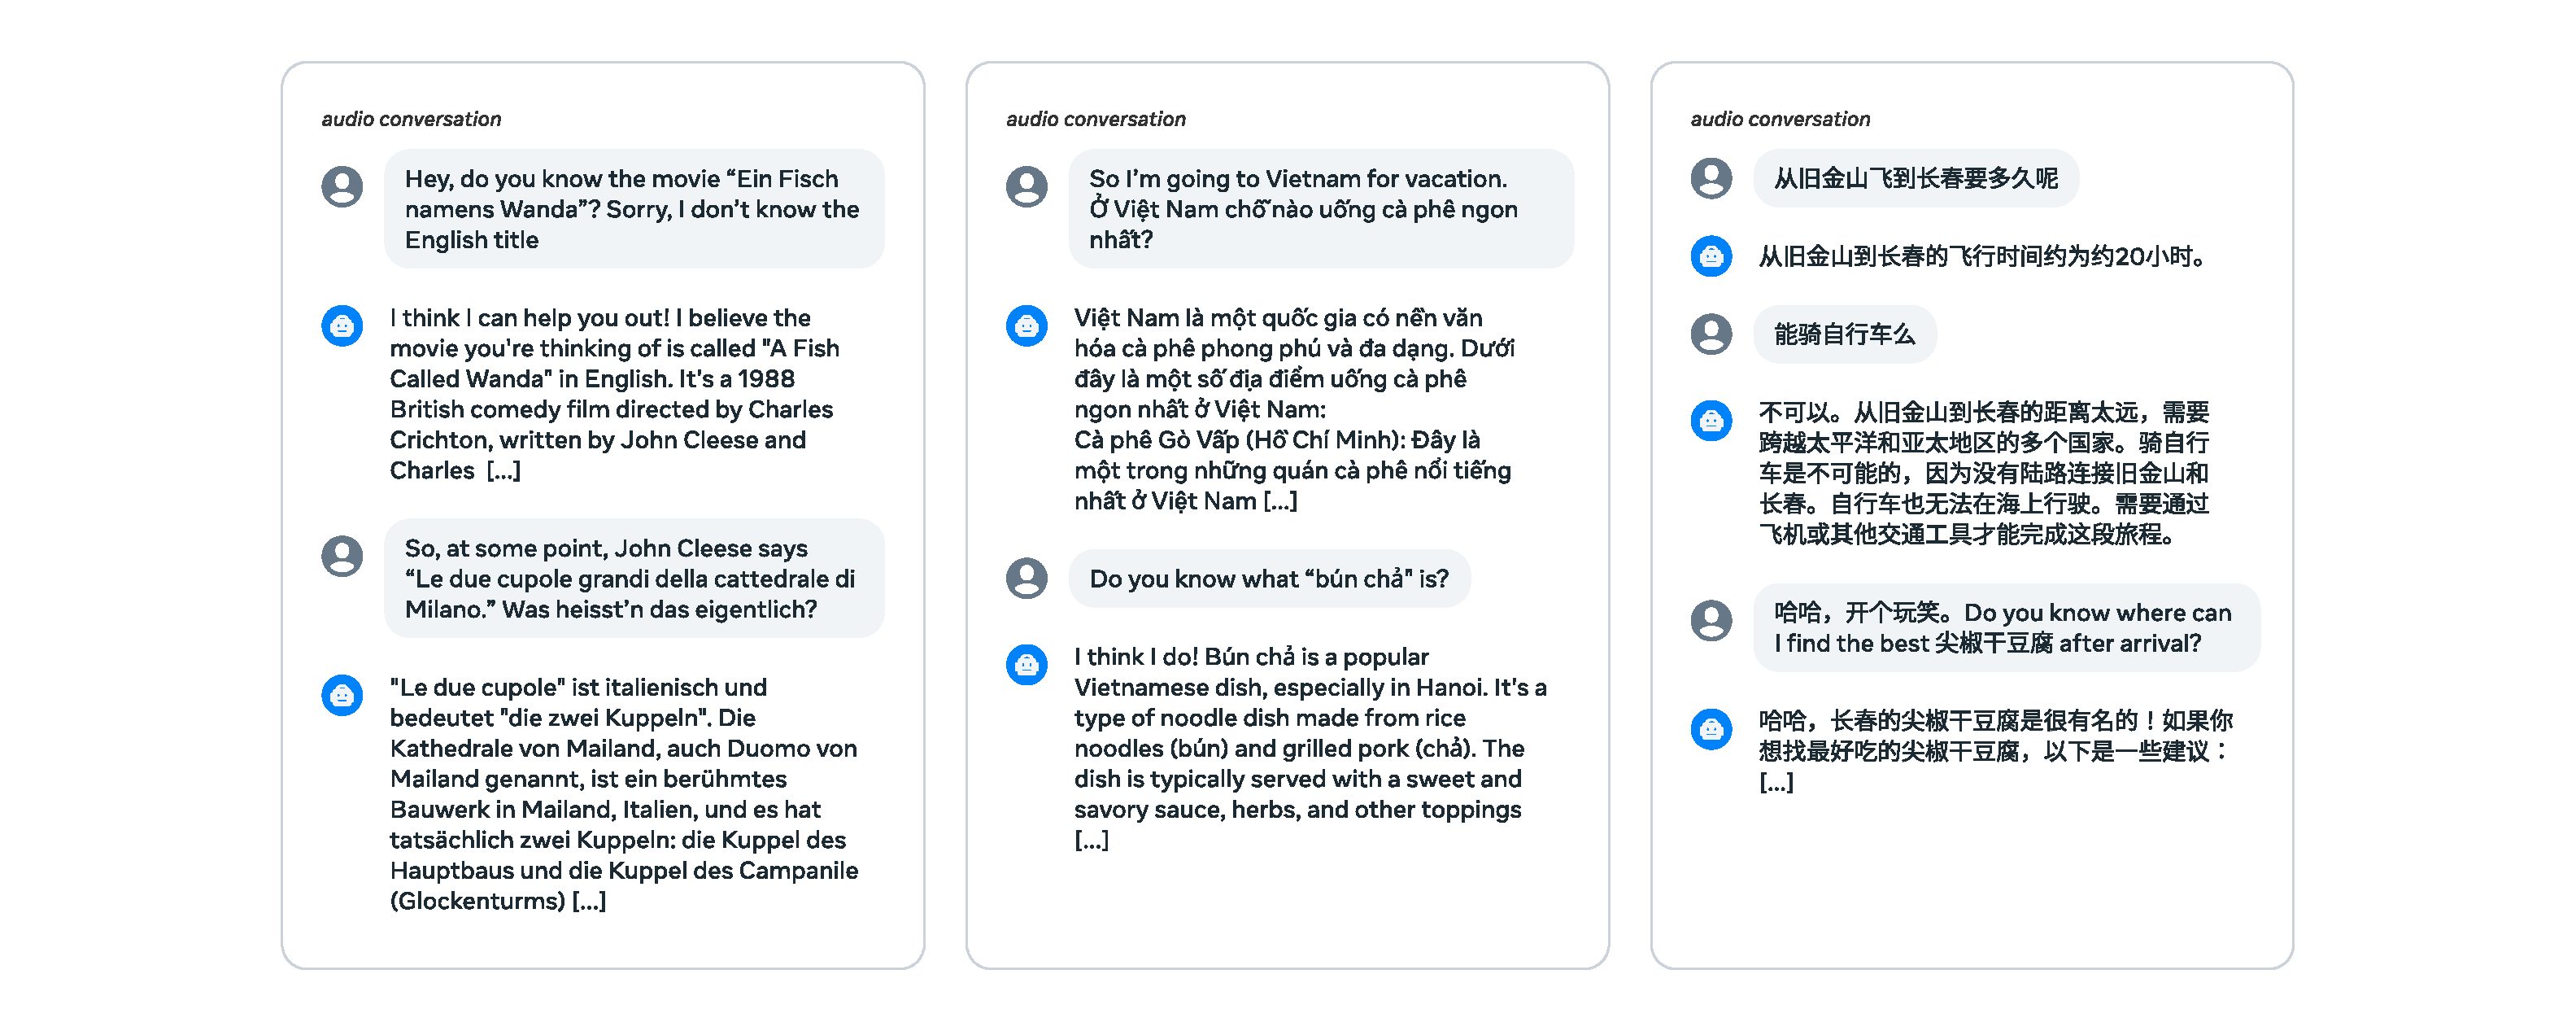
\includegraphics[trim={150px 0 150px 0},clip,width=\textwidth]{assets/llama-voice-language.pdf}
    \caption{\textbf{Transcribed dialogue examples using the speech interface for Llama 3.} The examples illustrate zero-shot multi-turn and code-switching capabilities.}
    \label{figure:speech_dialog_example}
\end{figure}

\textbf{Spoken question answering.}
The speech interface of Llama 3 demonstrates remarkable question answering capabilities. The model can effortlessly comprehend code-switched speech without any prior exposure to such data. Notably, although the model was trained only on single-turn dialogue, it is capable of engaging in extended, coherent multi-turn dialogue sessions.
Figure~\ref{figure:speech_dialog_example} presents a few examples that highlight these multilingual and multi-turn capabilities.

\begin{table}[t]
\centering
    \begin{tabular}{lcccccc}
    \toprule
     & \multicolumn{2}{c}{\textbf{Llama 3 8B}} &  \multicolumn{2}{c}{\textbf{Llama 3 70B}} & \multicolumn{2}{c}{\textbf{Gemini 1.5 Pro}} \\
    \textbf{Language} & AT \bdown & LT \bup & AT \bdown & LT  \bup & AT \bdown & LT \bup \\
    \midrule
    English & 0.84 & 15.09 & \textbf{0.68} & \textbf{15.46} & 1.44 & 13.42 \\
    Overall & 2.31 & 9.89 & \textbf{2.00} & 10.29 & 2.06 & \textbf{10.94} \\
    \bottomrule
    \end{tabular}
    \caption{\textbf{Speech toxicity of our speech interface to Llama 3 on the MuTox dataset.} AT refers to added toxicity (\%) and LT refers to lost toxicity (\%). \label{table:speech-safety-mutox}}
\end{table}

\textbf{Safety.}
We evaluate the safety of our speech model on MuTox \citep{mutox}, a multilingual audio-based dataset of 20,000 utterances for English and Spanish and 4,000 for 19 other languages, each with toxicity labels attached.
The audio is passed as input to the model and the output is evaluated for toxicity, after cleaning some special characters.
We apply the MuTox classifier~\citep{mutox} and compare the results with Gemini 1.5 Pro. We evaluate the percentage of added toxicity (AT), when the input prompt is safe and the output is toxic, and the percentage of lost toxicity (LT), when the input prompt is toxic and the answer is safe. Table~\ref{table:speech-safety-mutox} shows the results for English and an average across all 21 languages that we evaluated on.\footnote{Note that for Gemini, we encountered that a significant number of responses were empty, which could be due to safety filters on their side (though some empty responses were for non-toxic input) or to rate limits. To conduct the analysis, we assumed that all the empty responses are safe. This is the most conservative approach for results and the upper bound of what Gemini results would look like.} The percentage of added toxicity is very low: our speech models have the lowest percentage of added toxicity for English, with less than 1\%. It removes significantly more toxicity than it adds.


\subsection{Speech Generation Results}
For speech generation, we focus on evaluating the quality of token-wise input streaming models with the Llama 3 embeddings for the text normalization and prosody modeling tasks. The evaluation focuses on comparisons with models that do not take the Llama 3 embeddings as an additional input.

\textbf{Text normalization.}
To measure the effect of Llama 3 embeddings, we experimented with changing the amount of right context the model uses. We trained the model using a right context of 3 TN tokens (demarcated by unicode category). This model is compared to models that do not use the Llama 3 embeddings, using a 3-token right context or a full bi-directional context.
As expected, Table~\ref{tab:table1} shows using the full right context improves performance for the model without Llama 3 embeddings. However, the model that incorporates the Llama 3 embeddings outperforms all other models, hence enabling token-rate input/output streaming without relying on long context in the input.

\begin{wraptable}{r}{0.45\textwidth}
	\begin{NiceTabular}{lcc}
		\CodeBefore
		\Body
		\toprule
		\textbf{Model} & \textbf{Context} & \textbf{Accuracy} \\
		\midrule
		Without Llama 3 8B & 3 & 73.6\% \\
		Without Llama 3 8B & $\infty$ & 88.0\% \\
		With Llama 3 8B & 3 & \textbf{90.7\%} \\
		\bottomrule
	\end{NiceTabular}
	\caption{\textbf{Sample-wise text normalization (TN) accuracy.} We compare models with or without Llama 3 8B embeddings, and using different right-context values.\vspace{-8mm}}
	\label{tab:table1}
\end{wraptable}

\textbf{Prosody modeling.}
To evaluate the performance of the our prosody model (PM) with Llama 3 8B, we conducted two sets of human evaluation comparing models with and without Llama 3 embeddings. Raters listened to samples from different models and indicated their preferences. To generate the final speech waveform, we use an in-house transformer based acoustic model \citep{wu2021transformer} that predicts spectral features and a WaveRNN neural vocoder \citep{kalchbrenner2018efficient} to generate the final speech waveform.  %

\begin{table}[t]
	\centering
    \begin{minipage}{.48\textwidth}
      \centering
      \begin{tabular}{lcc}
		\toprule
		\textbf{Model} & \textbf{Preference} \\
		\midrule
		PM for Llama 3 8B  & \textbf{60.0\%} \\
		\small{Streaming phone-only baseline} & 40.0\% \\
		\bottomrule
      \end{tabular}
		\label{tab:tts:pm:ab_test1}
    \end{minipage}\hfill
    \begin{minipage}{.48\textwidth}
      \centering
      \begin{tabular}{lcc}
		\toprule
		\textbf{Model} & \textbf{Preference} \\
		\midrule
		PM for Llama 3 8B & \textbf{63.6\%} \\
		\small{Non-streaming phone-only baseline} & 36.4\% \\
		\bottomrule
      \end{tabular}

    \end{minipage}
    \caption{\textbf{Prosody Modeling (PM) evaluation.} \emph{Left:} Rater preferences of PM for Llama 3 8B vs. streaming phone-only baseline. \emph{Right:} Rater preferences of PM for Llama 3 8B vs. non-streaming phone-only baseline.}
    \label{tab:pm_test}

\end{table}




First, we compare directly to a streaming baseline model without Llama 3 embeddings. 
In  the second test, the Llama 3 8B PM is compared to a non-streaming baseline model without Llama 3 embeddings. 
As shown in Table~\ref{tab:pm_test}, the Llama 3 8B PM is preferred  60\% of the time compared to the streaming baseline, and 63.6\% of the time  compared to the non-streaming baseline, indicating a significant improvement in perceived quality. The key advantage of the Llama 3 8B PM is its token-wise streaming capability (Section~\ref{sec:tts:pm}), which maintains low latency during inference. This reduces the model's lookahead requirements, enabling more responsive and real-time speech synthesis compared to non-streaming baselines.
Overall, the Llama 3 8B prosody model consistently outperforms the baseline models, demonstrating its effectiveness in enhancing the naturalness and expressiveness of synthesized speech.

